% Created 2019-04-07 Sun 16:38
\documentclass[abstract=off,oneside]{scrreprt}
\usepackage[utf8]{inputenc}
\usepackage[T1]{fontenc}
\usepackage{fixltx2e}
\usepackage{graphicx}
\usepackage{longtable}
\usepackage{float}
\usepackage{wrapfig}
\usepackage{rotating}
\usepackage[normalem]{ulem}
\usepackage{amsmath}
\usepackage{textcomp}
\usepackage{marvosym}
\usepackage{wasysym}
\usepackage{amssymb}
\usepackage{hyperref}
\tolerance=1000
\usepackage{caption}
\usepackage{minted}
\author{Thomas Aven}
\date{\today}
\title{TDT4230 - Graphics and Visualization \large \\~\\ Final Project}
\hypersetup{
  pdfkeywords={},
  pdfsubject={},
  pdfcreator={Emacs 25.2.2 (Org mode 8.2.10)}}
\begin{document}

\maketitle

\section*{Introduction}
\label{sec-1}
I've been interested in the world of ray marching for a while, in
particular the fantastic work of Inigo Quilez (found at
\url{https://iquilezles.org/www/index.htm}). His blog explains an enormous
amount of techniques to create unbelievable procedural scenes, using
only a fragment shader. Most of these shaders are hosted at
Shadertoy.com, which is an online tool for sharing shaders with WebGL.
\\\\
My primary goal for this project thus became to create interesting
fragment shaders. This means that the only thing I'm allowed to pass
into the vertex shader is a \emph{single quad} that covers the
entire screen -- all the fragment shader has to work with is
\verb~gl_FragCoord~ (with some exceptions, more on that later).
\\\\
For this report I will go through the process step by step, from the
baby steps required to render a simple sphere, to the final leaps that
render a realistic looking scene. There are quite a few illustratory
images, which reside in the appendix, with links back and forth to
make the reading slightly less painful.

\section*{Building the project}
\label{sec-2}
The project uses CMake for the building process, as is required for
the assignment. I've also taken the liberty of adding three libraries
to use sound: OpenAL Soft , freealut and FFTW. OpenAL and freealut are
added as submodules with Git, while FFTW is added as an external
project in CMake, which fetches a tarball online, then extracts and
builds the library. Building thus takes a little while, but it's not
too painful. This has been tested with the package repositories found
in Ubuntu 18.04 and Debian Stretch, and should hopefully work right
out of the box.

\section*{Ray Marching}
\label{sec-3}
Now -- what is this ray marching thing? In the world of \emph{ray casting},
it is common to be familiar with \emph{ray tracing} to compute the
intersections of a light ray with surfaces. \emph{Ray marching} may be used
within such a ray tracing method, as it is a specific algorithm where
samples are taken along the direction of a ray to test for this
intersection. Using ray marching in combination with something that's
called \emph{signed distance functions} can make extraordinary
scenes from infinitesimal binary executables, as all that's required
are the underlying mathematical formulas.
\\\\
A signed distance function, let's say a sphere centered at the origin,
$f(x, y, z) = \sqrt{x^2 + y^2 + z^2} - 1$, for this example, can be
used to determine whether a point is inside or outside an object, as
well as the distance to the object if it is outside. This is in
contrast to more well known ray tracing implementations that have to
check for intersections with quite a lot of primitives (like
triangles).
\\\\
It's time for an example. In \verb~simple.frag~, there is a function,
\verb~sd_sphere~, that takes a point and a radius as arguments. Given this
point, the function will return the distance from a point \verb~p~ to a
sphere of radius \verb~r~ centered at the origin (the sphere can be
translated by translating \verb~p~). We can leverage this to draw the
sphere by sending out rays from our camera position, and iteratively
stepping forward by an amount equal to the closest object in the scene
(not necessarily found in the same direction of which we are
tracing). Below are two illustrations I have found to explain the
method the best.
\\\\
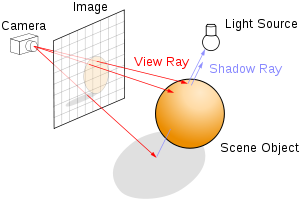
\includegraphics[width=0.45\textwidth]{./img/raytrace.png}
$\hspace{35pt}$
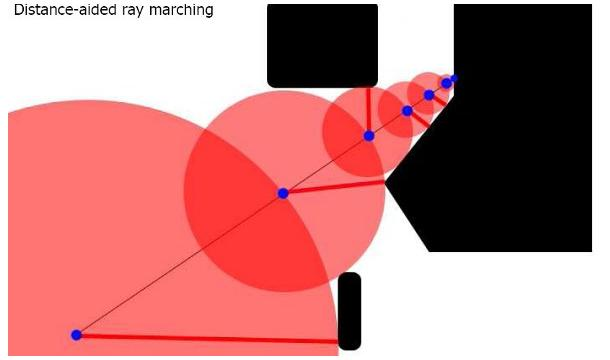
\includegraphics[width=0.45\textwidth]{./img/sphere_tracing.jpg}
\\\\
The left image (\url{http://jamie-wong.com/images/16-07-11/raytrace.png}),
shows how rays are traced from a camera. The right image
(\url{http://hugi.scene.org/online/hugi37/sphere_tracing.jpg}), illustrates
how the iterative steps are taken by the ray marching algorithm
according to the distance to the object closest to the current point.

\section*{Humble beginnings}
\label{sec-4}
\label{sec:beginnings}
Let's put our new knowledge to the test -- the execution of the ray
marching algorithm is found in any of the \verb~trace_<object>~
functions. A simple rendering of a sphere with some simple phong
shading is shown in \hyperref[fig:simplesphere]{this image}. Spheres are just the beginning, there
exists SDFs for a wide range of shapes:
\url{https://iquilezles.org/www/articles/distfunctions/distfunctions.htm}.

\section*{Setting the stage}
\label{sec-5}
\label{sec:creatingascene}
So we have a method of rendering a single object, in this case a
sphere. How do we go about turning this into a complex scene? The
first trick we will pull out of our sleeve is intersections and
unions. If we compute the distance to more than one object, and then
do \verb~max~ (intersect) or \verb~min~ between them, we can have multiple
objects in our scene. The technique can be seen in action \hyperref[fig:union]{here}.

\section*{Shadows}
\label{sec-6}
\label{sec:shadows}
An advantage of signed distance functions is that they provide us with
global information. Given a point on a surface in a scene, we can
fairly easily explore our surroundings -- we just have to recalculate
the SDF with new points. For shadowing, we simply follow what's called
a \emph{shadow ray} from the surface point towards the position of a given
light. If it intersects some other object on the way, the light will
not contribute to the illumination. We can also put areas that are
\emph{almost} within the shadow under penumbra by checking how close we are
to intersecting objects on the way. \hyperref[fig:penumbra]{Illustration}.

\section*{Sound and a Fast Fourier Transform}
\label{sec-7}
No shader is complete without its fft


\section*{Restrictions}
\label{sec-8}
\begin{itemize}
\item water looks like plastic with phong
\item numerical accuracy
\item glsl fucking sucks, stupid DSL
\item mapping a texture around a sphere >:(
\end{itemize}


$\pagebreak$
\section*{Appendix A - Images}
\label{sec-9}
\begin{figure}[htb]
\centering
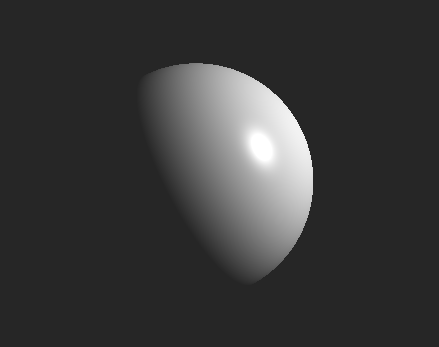
\includegraphics[width=0.70\textwidth]{./img/simplesphere.png}
\caption*{\label{fig:simplesphere}A simple ray marched sphere. \hyperref[sec:beginnings]{Back to section.}}
\end{figure}

\begin{figure}[htb]
\centering
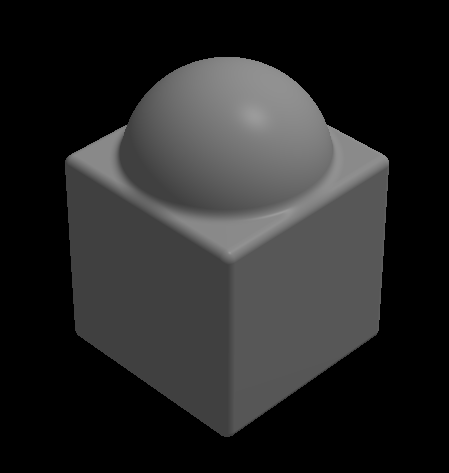
\includegraphics[width=0.70\textwidth]{./img/union.png}
\caption*{\label{fig:union}The union between a sphere and a cube. \hyperref[sec:creatingascene]{Back to section.}}
\end{figure}

\begin{figure}[htb]
\centering
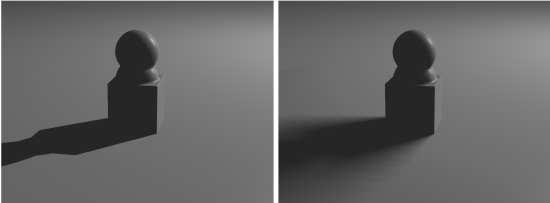
\includegraphics[width=0.99\textwidth]{./img/penumbra.png}
\caption*{\label{fig:penumbra}Penumbra shadowing in action. The left image has a \verb~k~-value of only 2, while the right image has a value of 128. \hyperref[sec:shadows]{Back to section.}}
\end{figure}
% Emacs 25.2.2 (Org mode 8.2.10)
\end{document}
